\section{Forward Kinematics of Mobile Robots}\label{sec:fwkmobile}
Whereas the pose of a robotic manipulator is uniquely defined by its joint angles---which can be made available using encoders in almost real-time---this is not the case for a mobile robot. Here, the encoder values simply refer to wheel orientation and need to be integrated over time, which will be a huge source of uncertainty as we will later see.
What complicates matters is that for so-called \emph{non-holonomic} systems, it is not sufficient to simply measure the distance that each wheel traveled, but also when each movement was executed. 

\begin{figure}[htb!]
	\centering
		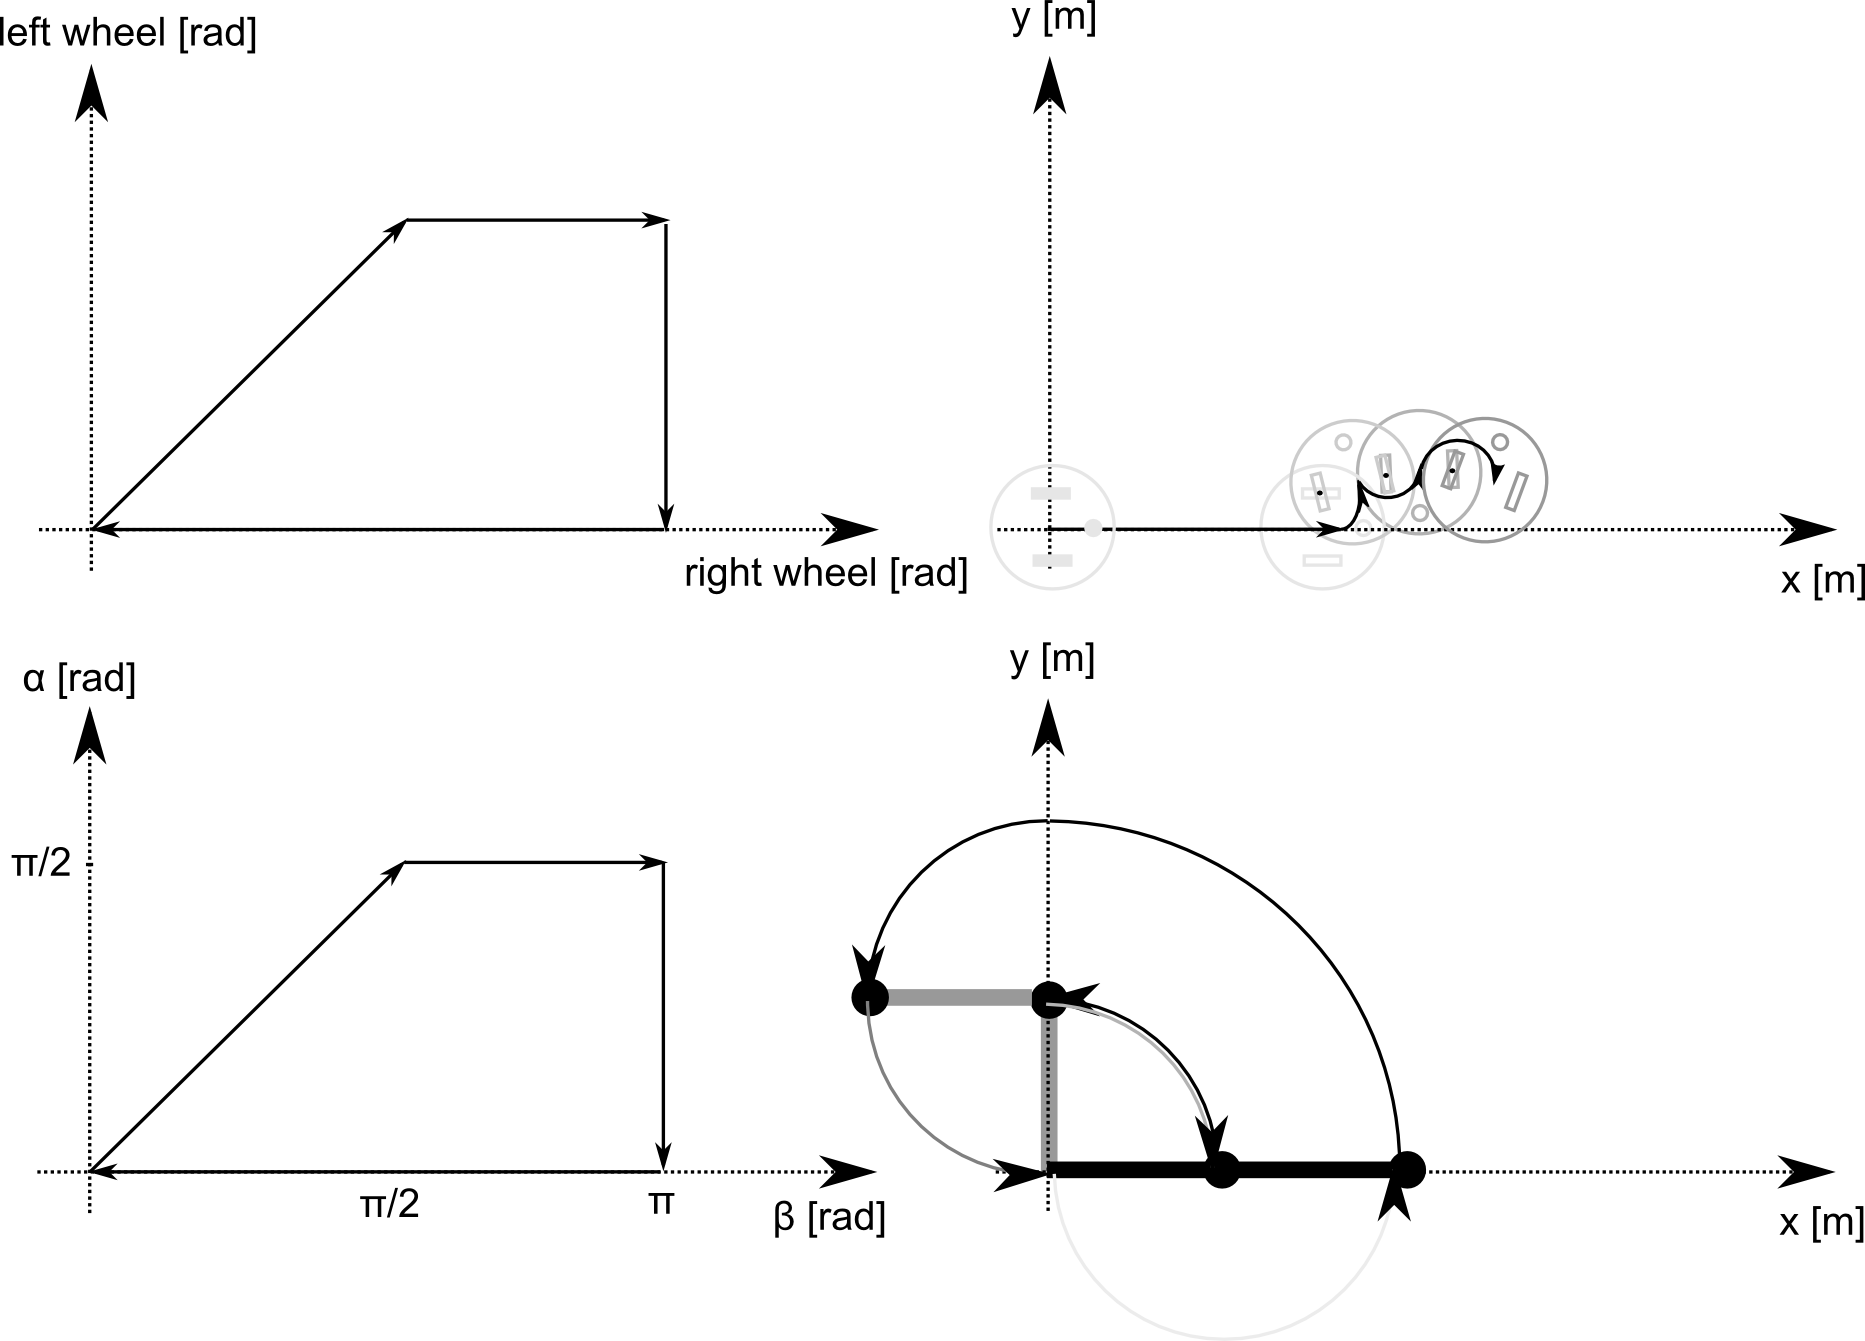
\includegraphics[width=0.95\textwidth]{figs/holonomy.png}
	\caption{Configuration space (left) and workspace (right) for a non-holonomic mobile robot (top) and a holonomic manipulator (bottom). Closed trajectories in configuration space result in closed trajectories in the workspace if the robot's kinematics is holonomic.}
	\label{fig:holonomy}
\end{figure}

A system is non-holonomic\index{Non-holonomic}\index{Holonomic} when closed trajectories in its configuration space (reminder: the configuration space of a two-link robotic arm is spanned by the possible values of each angle) may not have it return to its original state.  A simple arm is holonomic, as each joint position corresponds to a unique position in space. Going through whatever trajectory that comes back to the starting point in configuration space, will put the robot at the exact same position. A train on  a track is holonomic: moving its wheels backwards by the same amount they have been moving forward brings the train to the exact same position in space. A car and a differential-wheel robot are non-holonomic vehicles: performing a straight line and then a right-turn leads to the same amount of wheel rotation than doing a right turn first and then going in a straight line; getting the robot to its initial position requires not only to rewind both wheels by the same amount, but also getting their relative speeds right. The configuration and corresponding workspace trajectories for a non-holonomic and a holonomic robot are shown in Figure \ref{fig:holonomy}. Here, a robot first moves on a straight line (both wheels turn an equal amount). Then the left wheel remains fixed and only the right wheel turns forward. Then the right wheel remain fixed and the left wheel turns backward. Finally, the right wheel turns backward, arriving at the initial encoder values (zero). Yet, the robot does not return to its origin. Performing a similar trajectory in the configuration space of a two-link manipulator instead, let the robot return to its initial position. 

It should be clear by now that for a mobile robot, not only traveled distance per wheel matters, but also the speed of each wheel as a function of time. Instead, this information was not required to uniquely determine the pose of a manipulating arm. Lets introduce the following conventions. We will establish a world coordinate system $\{I\}$, which is known as the inertial frame by convention (Figure \ref{fig:mobilerobot}). We establish a coordinate system $\{R\}$ on the robot and express the robot's speed $^R\dot{\xi}$ as a vector $ ^R\dot{\xi}=[^R\dot{x}, ^R\dot{y}, ^R\dot{\theta}]^T$. Here $^R\dot{x}$ and $^R\dot{y}$ correspond to the speed along the x and y directions in $\{R\}$, whereas $^R\dot{\theta}$ corresponds to the rotation around the imaginary z-axis, that you can imagine to be sticking out of the ground. We denote speeds with dots over the variable name, as speed is simply the derivative of distance.  Think about the robot's position in $\{R\}$ real quick. It is always zero, as the coordinate system is fixed on the robot. Therefore, velocities are the only interesting quantities in this coordinate system and we need to understand how velocities in $\{R\}$ map to positions in $ \{I\}$, which we denote by $^I\xi=[^Ix, ^Iy, ^I\theta]^T$. These coordinate systems are shown in Figure \ref{fig:mobilerobot}. 

\begin{figure}[htb!]
	\centering
		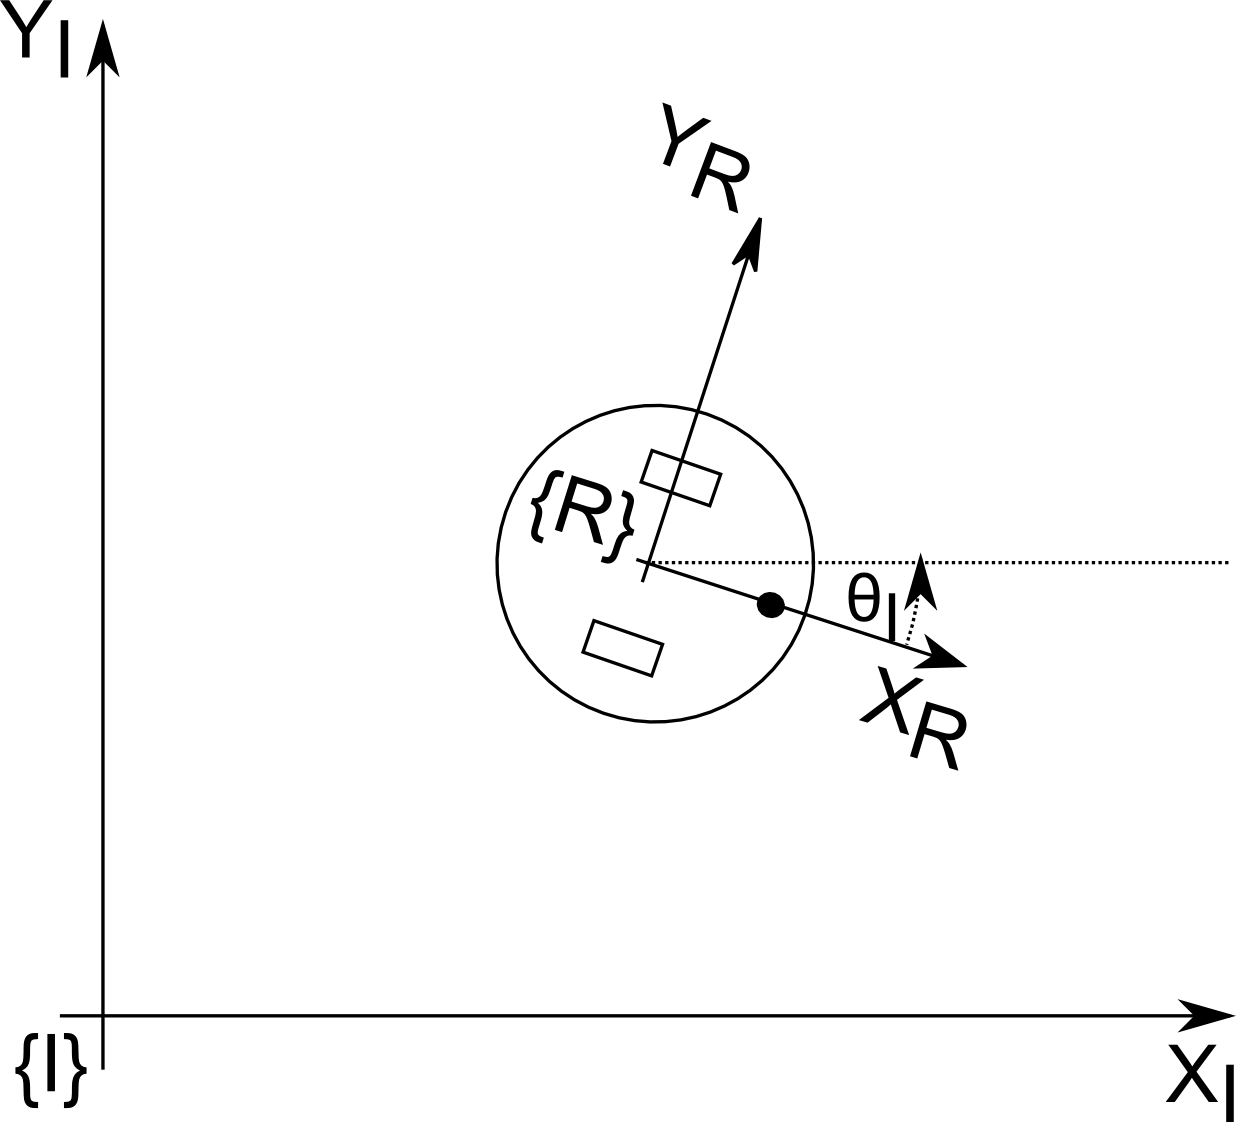
\includegraphics[width=0.85\textwidth]{figs/mobilerobot.png}
	\caption{Mobile robot with local coordinate system \{R\} and world frame \{I\}. The arrows indicate the positive direction of position and orientation vectors.}
	\label{fig:mobilerobot}
\end{figure}



Notice that the positioning of the coordinate frames and their orientation are arbitrary. Here, we chose to place the coordinate system in the center of the robot's axle and align $^Rx$ with its default driving direction.

In order to calculate the robot's position in the inertial frame, we need to first find out, how speed in the robot coordinate frame maps to speed in the inertial frame. This can be done again by employing trigonometry. There is only one complication: a movement into the robot's x-axis might lead to movement along both the x-axis and the y-axis of the world coordinate frame. By looking at the figure above, we can derive the following components to $\dot{x}_I$. First, 
\begin{equation}
\dot{x}_{I,x}=cos(\theta) \dot{x}_R.
\end{equation}

There is also a component of motion coming from $ \dot{y}_R$ (ignoring the kinematic constraints for now, see below).  For negative $ \theta$, as in Figure \ref{fig:mobilerobot}, a move along $y_R$ would let the robot move into positive $ X_I$ direction. The projection from $ \dot{y}_R$ is therefore given by 
\begin{equation}
\dot{x_{I,y}}=-sin(\theta)\dot{y_R}.
\end{equation} 
We can now write
\begin{equation}
\dot{x_I}=cos(\theta) \dot{x_R} - sin(\theta) \dot{y_R}.
\end{equation}
Similar reasoning leads to
\begin{equation}
\dot{y_I}=sin(\theta) \dot{x_R} + cos(\theta) \dot{y_R}
\end{equation}
and
\begin{equation}
\dot{\theta_I}=\dot{\theta_R}
\end{equation}
which is the case because both robot's and world coordinate system share the same z-axis in this example. We can now conveniently write
\begin{equation}
\dot{\xi_I}=^I_RT(\theta)\dot{\xi_R}
\end{equation}
with
\begin{equation}
^I_RT(\theta)=\left(\begin{array}{ccc}
cos(\theta) & -sin(\theta) & 0 \\
sin(\theta) & cos(\theta) & 0 \\
0 & 0 & 1\end{array}\right)
\end{equation}

We are now left with the problem of how to calculate the speed $ \dot{\xi_R}$ in robot coordinates. For this, we make use of the \emph{kinematic constraints}\index{Kinematic constraints} of the robotic wheels. For a standard wheel, the kinematic constraints are that every rotation of the wheel leads to strictly forward or backward motion and does not allow side-way motion or sliding. We can therefore calculate the forward speed of a wheel $ \dot{x}$ using its rotational speed $ \dot{\phi}$ (assuming the encoder value/angle is expressed as $ \phi$) and radius $ r$ by 
\begin{equation}
\dot{x}=\dot{\phi}r.
\end{equation}
This becomes apparent when considering that the circumference of a wheel with radius $ r$ is $ 2\pi r$. The distance a wheel rolls when turned by the angle $ \phi$ (in radians) is therefore $ x=\phi r$. Taking the derivative of this expression on both sides leads to the above expression.

\begin{figure}[htb!]
	\centering
		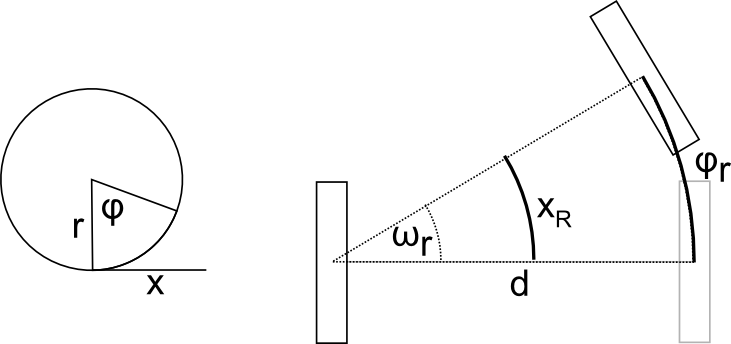
\includegraphics[width=0.9\textwidth]{figs/wheelrotation.png}
	\caption{Differential wheel robot pivoting around its left wheel.}
	\label{fig:wheelrotation}
\end{figure}

How each of the two wheels in our example contributes to the speed of the robot's center---where its coordinate system is anchored---requires the following trick: we calculate the contribution of each individual wheel while assuming all other wheels remaining un-actuated. In this example, the distance traveled by the center point is exactly half of that traveled by each individual wheel, assuming the non-actuated wheel rotating around its ground contact point (Figure \ref{fig:wheelrotation}). We can therefore write
\begin{equation}
\dot{x_R}=\frac{r\dot{\phi_l}}{2}+\frac{r\dot{\phi_r}}{2}
\end{equation}
given the speeds $ \dot{\phi_l}$ and $ \dot{\phi_r}$ of the left and the right wheel, respectively.

\begin{framed}
Think about how the robot's speed along its y-axis is affected by the wheel-speed given the coordinate system in the drawing above. Think about the kinematic constraints that the standard wheels impose.
\end{framed}

Hard to believe at first, but the speed of the robot along its y-axis is always zero. This is because the constraints of the standard wheel tell us that the robot can never slide. We are now left with calculating the rotation of the robot around its z-axis. That there is such a thing can be immediately seen when imaging the robot's wheels spinning in opposite directions. We will again consider each wheel independently. Assuming the left wheel to be non-actuated, spinning the right wheel forwards will lead to counter-clockwise rotation. Given an axle diameter (distance between the robot's wheels) $ d$, we can now write
\begin{equation}
\omega_r d = \phi_r r
\end{equation}
with $ \omega_r$ the angle of rotation around the left wheel (Figure \ref{fig:wheelrotation}, right). Taking the derivative on both sides yields speeds and we can write
\begin{equation}
\dot{\omega_r} = \frac{\dot{\phi_r} r}{d}
\end{equation}
Adding the rotation speeds up (with the one around the right wheel being negative based on the right-hand grip rule), leads to

\begin{equation}
\dot{\theta}=\frac{\dot{\phi_r} r}{d}-\frac{\dot{\phi_l} r}{d}
\end{equation}

Putting it all together, we can write

\begin{equation}
\left(\begin{array}{c} \dot{x_I}\\\dot{y_I}\\\dot{\theta}\end{array}\right)=\left(\begin{array}{ccc}
cos(\theta) & -sin(\theta) & 0 \\
sin(\theta) & cos(\theta) & 0 \\
0 & 0 & 1\end{array}\right)\left(\begin{array}{c}\frac{r\dot{\phi_l}}{2}+\frac{r\dot{\phi_r}}{2}\\0\\\frac{\dot{\phi_r} r}{d}-\frac{\dot{\phi_l} r}{d}\end{array}\right)
\end{equation}

\section{Inverse Kinematics of Mobile Robots}\label{sec:ivkmobile}
The main problem for the engineer is now to find out how to chose the control parameters to reach a desired position. This problem is known as inverse kinematics. Solving the inverse kinematics in closed form is not always possible, however. It can be done for the differential wheel platform we studied above. Lets first establish how to calculate the necessary speed of the robot's center given a desired speed $ \dot{\xi_I}$ in world coordinates. We can transform the expression $ \dot{\xi_I}=T(\theta)\dot{\xi_R}$ by multiplying both sides with the inverse of $ T(\theta)$:

\begin{equation}
T^{-1}(\theta)\dot{\xi_I}=T^{-1}(\theta)T(\theta)\dot{\xi_R}
\end{equation}
which leads to $ \dot{\xi_R}=T^{-1}(\theta)\dot{\xi_I}$. Here

\begin{equation}
T^{-1}=\left(\begin{array}{ccc}cos \theta & sin \theta & 0 \\ -sin \theta & cos \theta & 0 \\ 0 & 0 & 1\end{array}\right)
\end{equation}

which can be determined by actually performing the matrix inversion or by deriving the trigonometric relationships from the drawing.  Similarly, we can now solve

\begin{equation}
\left(\begin{array}{c} \dot{x_R}\\\dot{y_R}\\\dot{\theta}\end{array}\right)=\left(\begin{array}{c}\frac{r\dot{\phi_l}}{2}+\frac{r\dot{\phi_r}}{2}\\0\\\frac{\dot{\phi_r} r}{d}-\frac{\dot{\phi_l} r}{d}\end{array}\right)
\end{equation}

for $ \phi_l$, $ \phi_r$. (do this!) You will now see that your kinematic constraints actually render some desired velocities, namely those that would lead to non-negative $ \dot{y_R}$ unfeasible.


\section{Car-like steering}
Differential wheel drives are very popular in mobile robotics as they are very easy to build, maintain, and control. Although not holonomic, a differential drive can approximate the function of a fully holonomic robot by first driving on the spot to achieve the desired heading and then driving straight. Drawbacks of the differential drive are its reliance on a caster wheel, which performs poorly at high speeds , and difficulties in driving straight lines as this requires both motors to drive at the exact same speed.


These drawbacks are mitigated by car-like mechanisms, which are driven by a single motor and can steer their front wheels. This mechanism is known as ``Ackermann steering'' \index{Ackermann steering} and illustrated to the right. Ackermann steering should not be confused with ``turntable'' steering \index{Turntable steering} where the front wheels are fixed on an axis with central pivot point. Instead, each wheel has its own pivot point and the system is constrained in such a way that all wheels of the car drive on circles with a common center point, avoiding skid.

\subsection{Forward Kinematics of Ackermann Steering}
As the Ackermann mechanism lets all wheels drive on circles with a common center point, its kinematics can be approximated by those of a tricycle with rear-wheel drive.

Let the car have the shape of a box with length $ L$ between rear and front axis. Let the center point of the common circle described by all wheels be distance $ R$ from the car's longitudinal center line.  Then, the steering angle $ \phi$ is given by

\begin{equation}
\tan \phi = \frac{L}{R}
\end{equation}


\subsection{Coordinate frames for a simplified car-like steering}
Let the robot coordinate system $ (x_r,y_r,\theta_r)$ be centered on the car's rear axis. Then, $ \dot{x}_r$ is the car's speed given by the speed of the car's engine. We can now derive expressions for the car's position in world coordinates $ (x_w,y_w,\theta_w)$.  (Remember: as the car is non-holonomic we can derive the kinematics only for speeds, the derivative of position, without integrating.)

\begin{eqnarray}
\dot{x}_w&=&\cos{\theta_w}\dot{x}_r\\
\dot{y}_w&=&\sin{\theta_w}\dot{x}_r\\
\dot{\theta}_w&=&\frac{\tan{\phi}}{L}\dot{x}_r
\end{eqnarray}

The last expression directly follows from the rule that the tangent of an angle is equivalent to the ratio of its opposite to adjacent edges. At this point it is worth recalling that $ \dot{y}_r=0$, no matter what, as a simple model does not allow the robot to skid. Therefore, the steering angle $ \phi$ only affects the rotation of the car.

At this point, you have expressions for predicting the movement of the car's bounding box through space as a function of speed and steering angle. The angles of the left and the right wheel, $ \phi_l$ and $ \phi_r$ can be calculated using the fact that all wheels of the car rotate around circles with a common center point. With the distance between the two front wheels $ l$, we can therefore write

Angles of individual wheels for perfect Ackermann steering
\begin{eqnarray}
\frac{L}{R-l/2}&=\tan{(\pi/2-\phi_r)}\\
\frac{L}{R+l/2}&=\tan{(\pi/2-\phi_l)}
\end{eqnarray}
with $ R=L\tan{\phi}$, again following the rule tangent = opposite / adjacent. This is important to calculate the resulting wheel angles and to test whether they are within the constraints of the actual vehicle.
